\section{POISE for ESR}
\label{sec:poise__esrpoise}

In the final section of this chapter, I briefly discuss how the concept of on-the-fly optimisation may be extended to pulsed ESR spectroscopy as well.
Much of the underlying code from (NMR-)POISE was recycled for this, including the implementation of the three optimisation algorithms (NM, MDS, and BOBYQA).
I added only one small difference in ESR-POISE, namely, a way to control the initial size of the simplex (for NM and MDS) or the trust region radius (for BOBYQA): in NMR-POISE, this is fixed at ten times the desired optimisation tolerance.
The overall optimisation framework (\cref{fig:poise_flowchart}), as well as the concept of the optimisation routine (\cref{subsec:poise__routines}), are retained: this preserves the generality of POISE, which is probably its greatest strength.

Naturally, TopSpin-specific sections of the code had to be rewritten to instead be compatible with Bruker's Xepr software.
This in fact proved to be easier than anticipated: most of the TopSpin code could be completely deleted, because Xepr provides an API which can be accessed from external programmes such as Python 3.
Thus, ESR-POISE is in fact completely written in Python 3, and there is no need for an artificial separation between `frontend' and `backend' (which also neatly circumvents most of the issues discussed in \cref{subsec:poise__implementation}).
The Xepr-facing code was written by \JBV{} (University of Oxford) and David Goodwin (University of Southampton, formerly Oxford).

A number of applications in ESR-POISE were explored.
All ESR experimental work was done by \JBV{} and William Myers (Oxford); thus, I only provide very brief descriptions here.
The examples include:

\begin{itemize}
    \item optimisation of the signal phase in a simple spin echo experiment, by maximising the intensity of the detected echo;
    \item similarly, calibration of \ang{90} and \ang{180} pulse widths and powers in a spin echo;
    \item optimisation of an inversion pulse used on the pump channel in a DEER experiment\autocite{Pannier2000JMR}, in order to increase the modulation depth of the resulting DEER traces (which reveal dipolar couplings between electrons);
    \item calibration of shaped pulse amplitudes for CHORUS broadband excitation\autocite{Foroozandeh2019JMR,Verstraete2021JCP};
    \item compensation for resonator distortions when applying shaped pulses, again demonstrated using the CHORUS sequence.
\end{itemize}

An example of the results obtained via the latter two optimisations is shown in \cref{fig:esrpoise_comp}.
In \cref{fig:esrpoise_comp_nocomp}, the CHORUS broadband excitation experiment was run without any optimisations: the resulting spectrum (blue, solid) is compared against that obtained via a standard field sweep (grey, dashed).
Clearly, there are substantial mismatches.
\Cref{fig:esrpoise_comp_ampcomp} shows the improved performance of CHORUS after a simple optimisation of the shaped pulse amplitudes, using the spectral intensity (or the negative thereof, since we seek to maximise it) as the cost function: the POISE optimisation therefore allows for a much more accurate spectrum to be obtained.

This can be further improved, however, by compensating for distortions in the pulse shape caused by the resonator.
Typically, this is a time-consuming process, requiring the determination of a transfer function: in this case, however, it can be performed in a fully automated fashion using POISE.
The coefficients in the transfer function are used as optimisation parameters, and are used within each function evaluation to back-calculate a compensated pulse shape: the cost function used is the difference between the compensated CHORUS spectrum and the field sweep ($f_\text{diff}$, as defined in \cref{eq:ps_cf_diff}).
At the point where the cost function is minimised, the transfer function parameters will have been accurately determined.
The final compensated CHORUS spectrum is shown in \cref{fig:esrpoise_comp_resoncomp}.

\begin{figure}[htb]
    \centering
    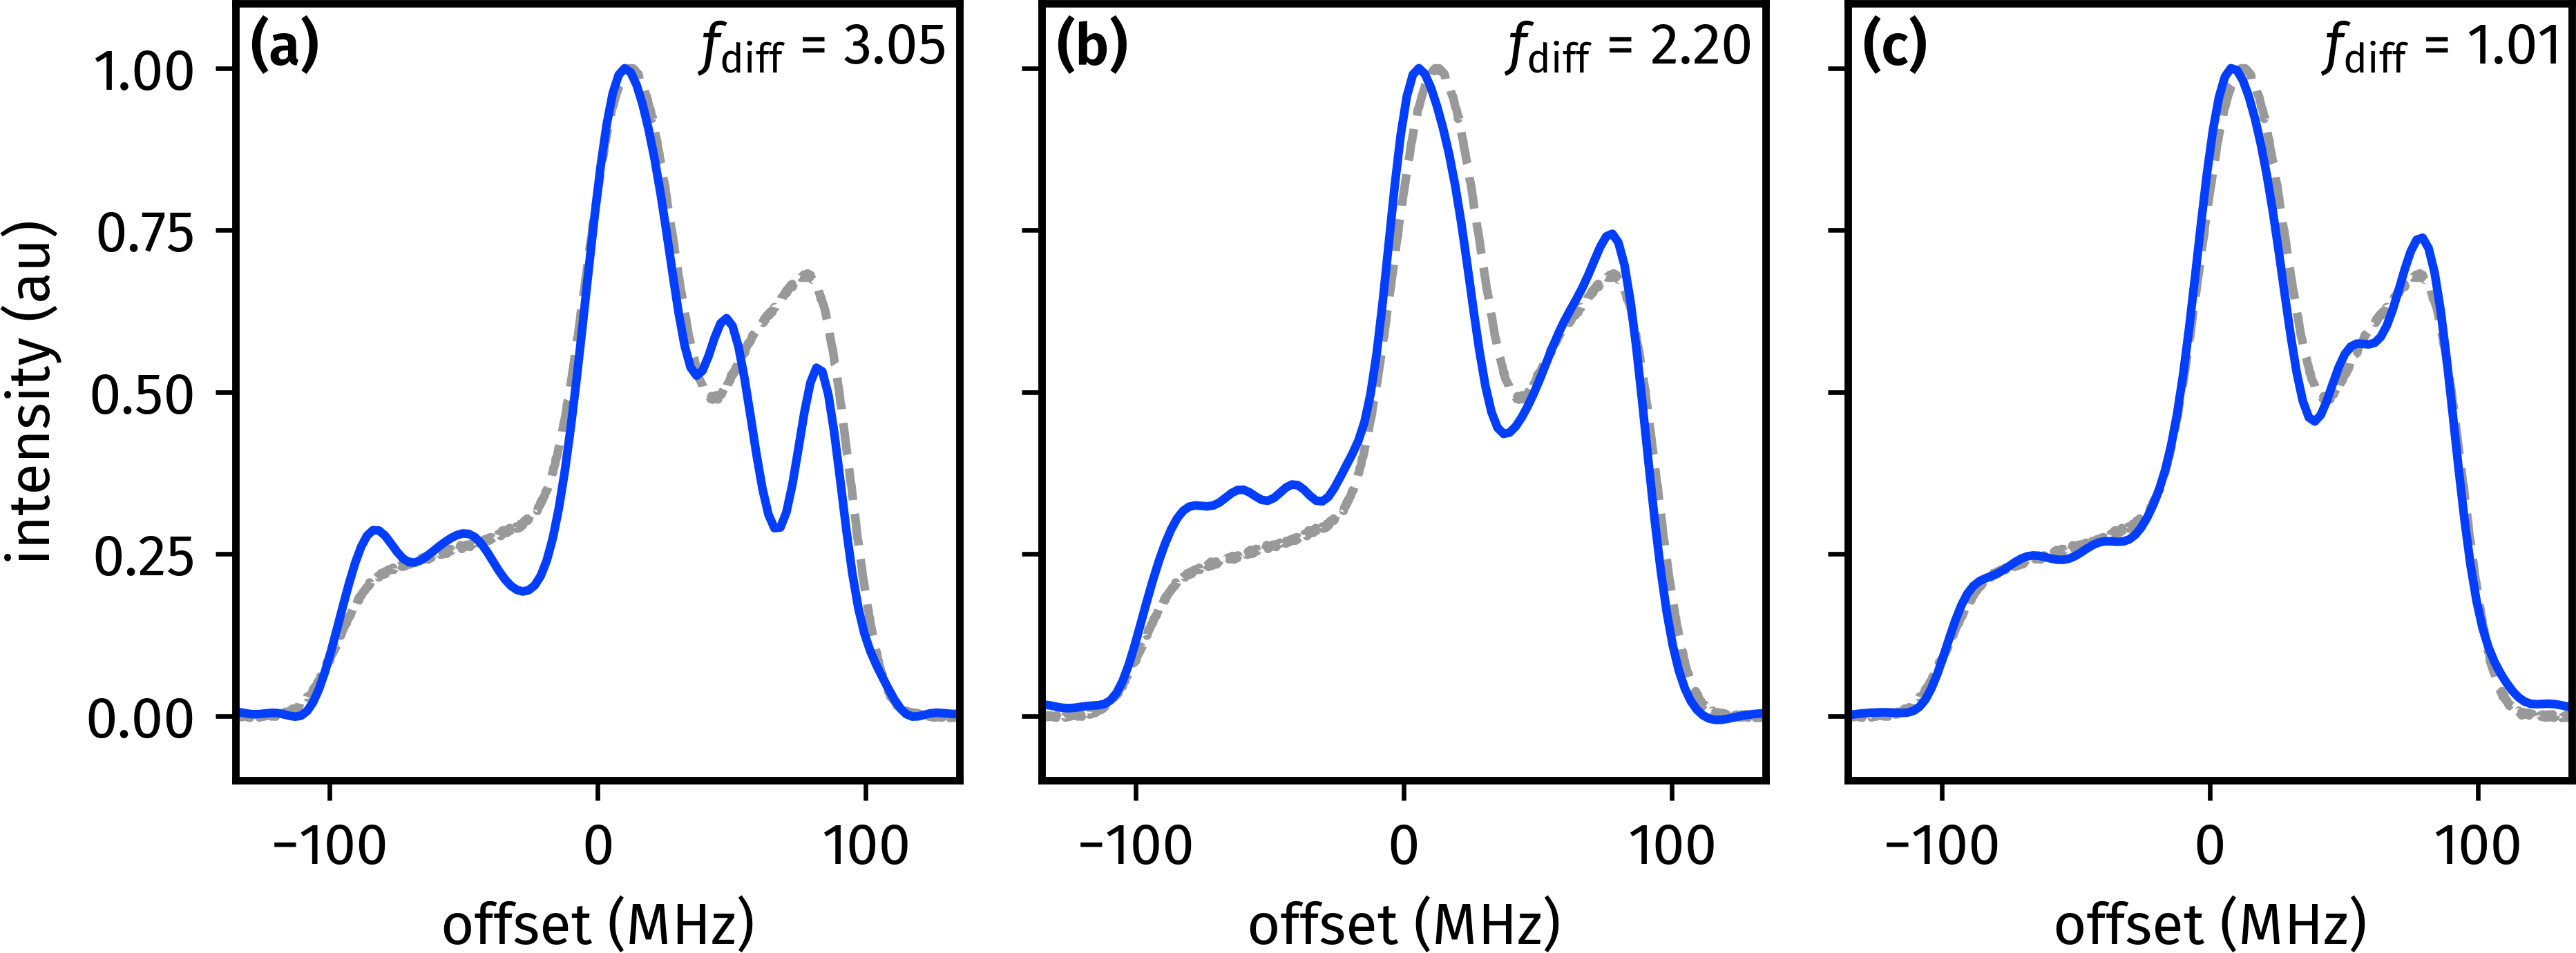
\includegraphics[]{poise/esrpoise_comp.png}%
    {\phantomsubcaption\label{fig:esrpoise_comp_nocomp}}%
    {\phantomsubcaption\label{fig:esrpoise_comp_ampcomp}}%
    {\phantomsubcaption\label{fig:esrpoise_comp_resoncomp}}%
    \caption[Comparison between CHORUS spectrum and field sweep before and after optimisation]{
        Comparison between CHORUS spectrum (blue, solid line) and field sweep profile (grey, dashed line):
        \textbf{(\subref*{fig:esrpoise_comp_nocomp})} without any optimisation of CHORUS,
        \textbf{(\subref*{fig:esrpoise_comp_ampcomp})} after optimisation of the CHORUS amplitudes, and
        \textbf{(\subref*{fig:esrpoise_comp_resoncomp})} using a compensated CHORUS pulse obtained through determination of the resonator transfer function.
        The value of $f_\text{diff}$ is indicated on each plot.
        The sample used was a bisnitroxide; further experimental details are provided in the paper.\autocite{Verstraete2022CC}
        The data used for this figure were acquired by \JBV{}.
    }
    \label{fig:esrpoise_comp}
\end{figure}
